\paragraph{How much evidence suffices for a fixed-pool decision?}
Sequential disclosure asks when the same fixed comparison becomes decidable. The 26 eligible classification tasks contain $43{,}007$ canonical labels: $20$ binary AUC tasks and six multiclass log-loss tasks. We use each task's first common metadata-ordered split and the same Mitra\_GPU/LightGBM predictions. Archived labels are masked and disclosed under the fixed metric and completion domain.

Under the same strict completion rule, random disclosure needs $95.76\%$ of each pool on average, compared with $92.15\%$ for predictive entropy, $77.97\%$ for interval width, $68.67\%$ for fixed expected gain and $65.44\%$ for adaptive expected gain (Fig.~\ref{fig:disclosure}). The adaptive rule requires fewer labels than the mean random path on all 26 fixed pools. The mean absolute reduction is $30.32$ percentage points; the mean of the per-task relative reductions is $32.09\%$. These two summaries use different denominators. All $1{,}404$ paths terminate at a correct certificate for the fully disclosed pool.

\begin{figure}[t]
\centering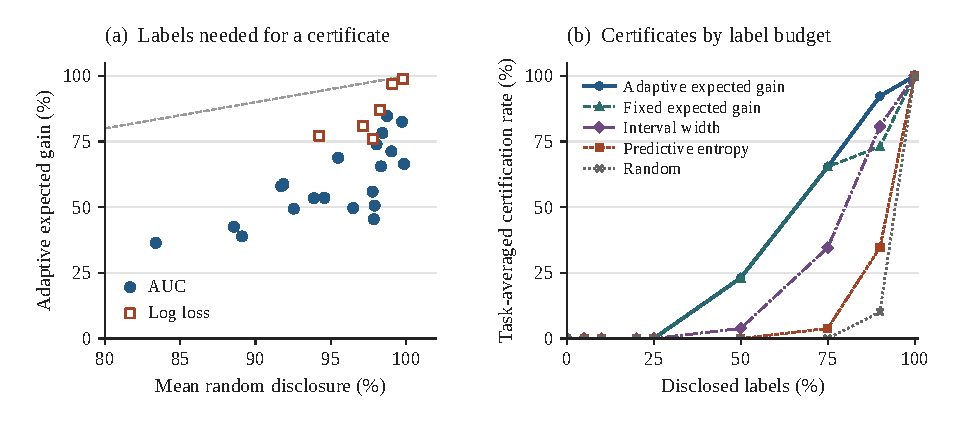
\includegraphics[width=\textwidth]{figures/sequential_disclosure.pdf}
\caption{\textbf{Decision-certified disclosure on frozen prediction pools.} \textbf{(a)} Label fractions required by adaptive expected gain and mean random disclosure, with one point per task. \textbf{(b)} Task-averaged certification rates at the recorded label budgets. Counts concern existing archived labels. Fixed predictions, canonical row identities, a shared completion domain and the same stopping rule are held constant across policies.}
\label{fig:disclosure}
\end{figure}

The pooled result covers distinct regimes: adaptive disclosure averages $59.21\%$ for AUC and $86.20\%$ for log loss. It is also prior-sensitive. Post hoc replacement of the pooled probability prior gives $63.81\%$ with Mitra probabilities, $73.06\%$ with LightGBM probabilities and $77.97\%$ with uniform class probabilities. Mitra wins 23 of these 26 complete-pool comparisons; its prior improves 17 acquisition paths, leaves two unchanged and worsens seven. These results describe this model collection and do not select a new prior using the test outcomes.

Two separate numerical controls support the stopping certificates. Generic same-domain LPs agree on 104 endpoints before and at adaptive stopping, with maximum difference $5.68\times10^{-14}$. A separate exact-arithmetic implementation imports neither the production policy nor its bound and stopping routines; it reproduces all $1{,}404$ paths and verifies $2{,}808$ stopping-prefix checks. Re-execution of the scoped VMA query-function adapter reproduces all $600$ frozen control paths byte for byte. On six log-loss tasks that function requires $97.72\%$ of labels versus $97.75\%$ for its matched random sampler under the same strict certificate. The six-task hindsight minimum averages $78.09\%$; it uses all answers. Section~S23 gives the task-level results and precise query-function scope, including its distinction from the full VMA/LURE procedure.

Collectively, these results demonstrate that strict decision certificates emerge substantially before full pool disclosure, while decoupling heuristic acquisition policies from the policy-agnostic algebraic verifier and its source-bound budget record.